% Idea general

% \begin{itemize}
%     \item Parser C3D
%     \item Entorno Bevy
%     \item creación configuraciones (toml)
% \end{itemize}


\chapter{Desarrollo} \label{sec:cap3}

\noindent Este proyecto se ha llevado a cabo en diferentes etapas. En un comienzo, se trabaja con un fichero \ac{C3D} capturado por las cámaras de INEF, con el sistema de captura de datos de la marca Vicon explicado en el \autoref{sec:cap2}. Estos datos de entrada consisten en una grabación a 240 Hz de un \textit{swing} de golf\footnote{Un swing de golf es la acción mediante la cual los jugadores golpean la pelota en este deporte \autocite{GolfSwing2025}}. 

Como se ha explicado en el \autoref{sec:ficheros-c3d}, un \ac{C3D} es un fichero binario que contiene la posición de diferentes marcadores en el tiempo. Por tanto, no es difícil convertir estos datos en un formato de texto legible. Se muestra en la \autoref{tab:c3d_data} un fragmento de un fichero \ac{C3D} que se ha utilizado durante el desarrollo de la aplicación convertido a una tabla:

\begin{table}[htbp]
  \centering
  \setlength{\tabcolsep}{5pt}
  \renewcommand{\arraystretch}{1.2}
  \rowcolors{3}{white}{gray!10}
  \begin{tabular}{r|S[table-format=-3.2]S[table-format=-3.2]S[table-format=-3.2]|S[table-format=-3.2]S[table-format=-3.2]S[table-format=-3.2]}
  \toprule
  \multirow{2}{*}{\textbf{Frame}} & \multicolumn{3}{c|}{RFIN                          } & \multicolumn{3}{c}{RFRA                          } \\
    & {\textbf{x}} & {\textbf{y}} & {\textbf{z}} & {\textbf{x}} & {\textbf{y}} & {\textbf{z}} \\
  \midrule
  1 & 46.80 & 3.25 & 664.41 & -23.14 & -4.06 & 827.33 \\
  2 & 46.80 & 3.25 & 664.41 & -23.14 & -4.07 & 827.30 \\
  3 & 46.80 & 3.25 & 664.41 & -23.14 & -4.08 & 827.30 \\
  4 & 46.80 & 3.25 & 664.41 & -23.14 & -4.07 & 827.30 \\
  5 & 46.80 & 3.25 & 664.41 & -23.15 & -4.06 & 827.31 \\
  \midrule
  6 & 46.80 & 3.25 & 664.41 & -23.16 & -4.03 & 827.33 \\
  7 & 46.81 & 3.25 & 664.41 & -23.18 & -4.00 & 827.35 \\
  8 & 46.82 & 3.28 & 664.40 & -23.21 & -3.99 & 827.36 \\
  9 & 46.87 & 3.36 & 664.40 & -23.23 & -4.02 & 827.33 \\
  10 & 46.93 & 3.51 & 664.38 & -23.23 & -4.09 & 827.26 \\
  \bottomrule
  \end{tabular}
  \caption{Fragmento de un fichero C3D convertido a tabla}
  \label{tab:c3d_data}
\end{table}

Se puede observar que aparecen dos marcadores, \ac{RFIN} y \ac{RFRA}, con sus coordenadas en el espacio, representadas por los valores de las columnas \textit{x}, \textit{y} y \textit{z}, en unidades de milímetros.

\section{\textit{Parser} \acs{C3D}} \label{sec:parser-c3d}
Estos datos se deben integrar con el resto del programa. Para ello, se debe contar con un \textit{parser} que convierta trate con el binario.

Se ha partido del \textit{crate} de \textit{Rust} \texttt{bevy-c3d}. Este \textit{crate} utiliza a su vez el \textit{crate} \texttt{c3dio}, que es un \textit{parser} para ficheros \ac{C3D}, pero integrado a \textit{Bevy}. De este modo, se consigue un \textit{Asset} que se puede cargar en el motor de juego.

Se ha modificado el \textit{crate} \texttt{c3dio} para adaptarlo a las necesidades del proyecto. En este caso, se han arreglado dos errores graves que impiden la compatibilidad con los ficheros generado por Vicon. Ambos errores se deben a modificaciones en la especificación introducidos de manera unilateral por Vicon. El primero de ellos se debe a una modificación en la especificación que cambia la manera de codificar los eventos, que hace que no se lea ningún evento del \ac{C3D}. El segundo error se debe a que Vicon elimina una restricción de la especificación, que limita el número de marcadores a 255. En este caso, Vicon permite un número ilimitado de marcadores, lo que provoca que el \textit{parser} solo reconozca los primeros 255 marcadores, y el resto no se lean.   

\section{\textit{Bevy}} \label{sec:bevy}
Este proyecto usa el motor de videojuegos \textit{Bevy} como base para generar un entorno tridimensional donde representar el \ac{C3D}. Bevy sigue el paradigma \ac{ECS}. \todo{Referencia}

Se muestra en la \autoref{fig:entorno3D} una imagen del entorno tridimensional creado con Bevy, antes de cargar el \ac{C3D}.


\begin{figure}[H]
  \centering
  \includegraphics[width=\textwidth]{imagenes/entorno3D.png}
  \caption{Entorno 3D creado con Bevy (modo oscuro)}
  \label{fig:entorno3D}
\end{figure}

En este entorno destacan el plano central, representado en un color verde oscuro, y sobre el que se apoyan 3 vectores que sirven como referencia. El código que genera estos vectores se incluye en el \autoref{apx:spawn_ref_vec}, demostrando la flexibilidad de \textit{Bevy} y el potencial de Rust. 

El pequeño botón que aparece en la esquina superior izquierda permite cambiar el color de fondo, alternando entre un modo claro y un modo oscuro. En la \autoref{fig:modo_claro} se muestra el entorno en modo claro. Variar entre estos modos permite mejorar el contraste con los marcadores, y por tanto, mejorar la visibilidad de los mismos.

\begin{figure}[H]
  \centering
  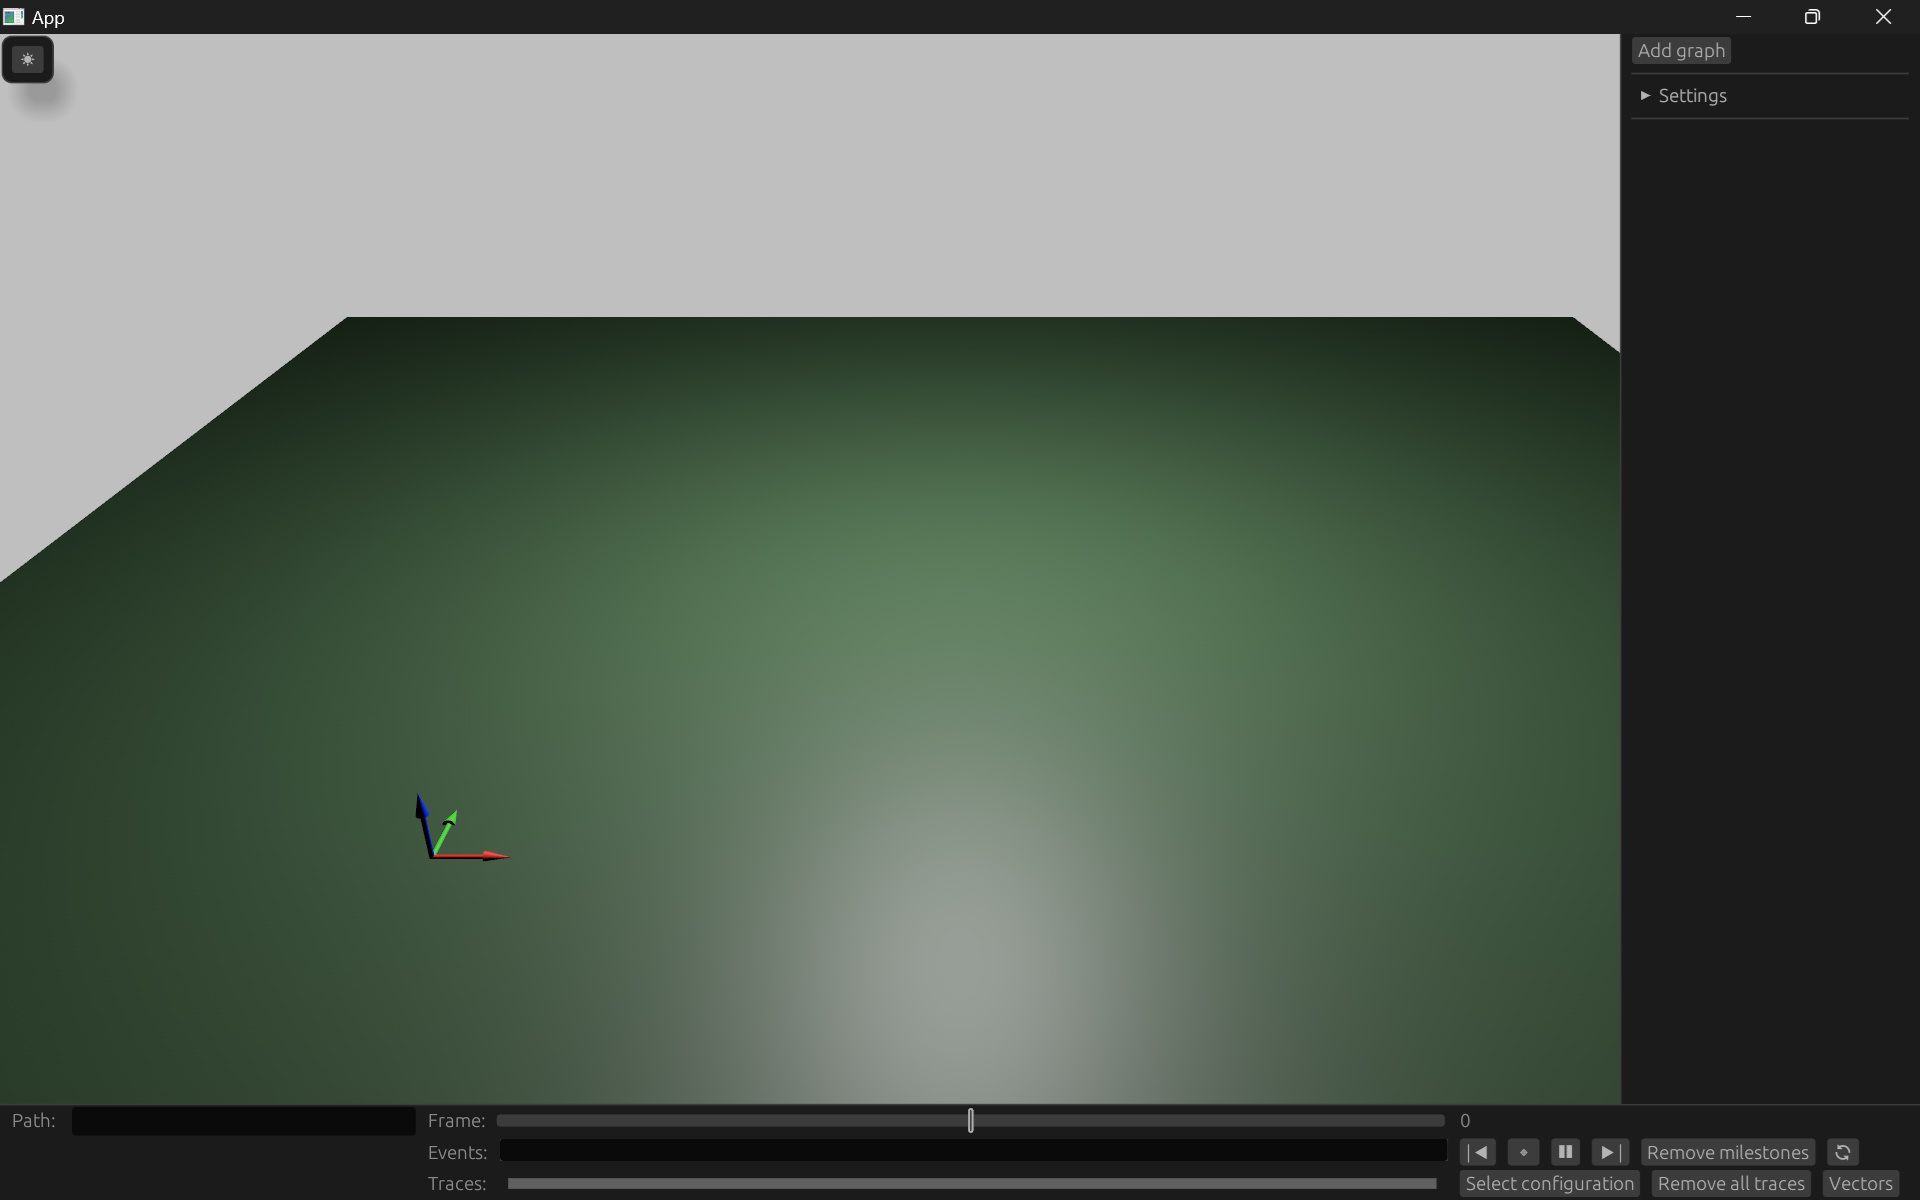
\includegraphics[width=\textwidth]{imagenes/modo_claro.png}
  \caption{Entorno en modo claro}
  \label{fig:modo_claro}
\end{figure}

\subsection{Información global} \label{sec:bevy-global}

El programa almacena una serie de información a partir del \ac{C3D} cargado. Esta información se almacena en un \texttt{Resource}, que es una estructura de datos que permite gestionar y acceder a la información de manera eficiente. Esta estructura tiene el nombre de \texttt{AppState}, y contiene la información global necesaria para el funcionamiento del programa. Esta información incluye el \textit{frame} actual, el número de \textit{frames} del \ac{C3D}, el \textit{path} al fichero \ac{C3D}, el \textit{path} al fichero de configuración, la tasa de refresco del \ac{C3D}, la tasa de refresco seleccionada por el usuario, y diferentes booleanos que contienen información sobre el estado del programa, como si se está reproduciendo o no.


\subsection{Orientación a eventos} \label{sec:bevy-eventos}

Este proyecto tiene un enfoque orientado a eventos. Esto significa que el programa reacciona a los eventos que ocurren en el entorno, como la carga de un fichero o la interacción del usuario. Un evento en \textit{Bevy} es una estructura de datos que representa una acción o un cambio en el estado del programa. Estos eventos pueden ser generados por el usuario, como pulsar un botón o mover el ratón, o por el propio programa, como la carga de un fichero o la actualización de la escena. Cuando ocurre un evento, \textit{Bevy} reacciona en la siguiente iteración de su bucle interno, lo que implica que tiene efecto en la siguiente actualización de la imagen, que típicamente coincidirá con el siguiente \textit{frame}.

Los eventos definidos en este proyecto se agrupan en seis enumerados, que se reúnen en la \autoref{tab:enum-eventos}:

\begin{table}[H]
  \centering
  % \setlength{\tabcolsep}{5pt}
  \rowcolors{2}{white}{gray!10}
  \begin{tabular}{c|c}
  \toprule
  {\textbf{Grupo}} & {\textbf{Relación}} \\
  \midrule
  MarkerEvent & Marcadores \\
  JoinsEvent & Uniones \\
  VectorEvent & Vectores \\
  TraceEvent & Trazas \\
  MilestoneEvent & Eventos \\
  GraphEvent & Interfaz gráfica \\
  \bottomrule
  \end{tabular}
  \caption{Grupos de eventos definidos en el programa}
  \label{tab:enum-eventos}
\end{table}

Cada grupo de eventos cuenta con un orquestador encargado de tomar las acciones pertinentes dependiendo del subtipo de evento. Rust facilita el manejo de eventos de este tipo, puesto que cada grupo se codifica como un \texttt{enum}, que define diferentes variantes.

En resumen, los eventos definidos en el programa se agrupan en la \autoref{tab:eventos}:

\begin{table}[H]
  \centering
  % \setlength{\tabcolsep}{5pt}
  \rowcolors{2}{white}{gray!10}
  \begin{tabular}{c|c}
  \toprule
  {\textbf{Evento}} & {\textbf{Significado}} \\
  \midrule
  DespawnAllMarkersEvent & Elimina todos los marcadores \\
  DespawnAllJoinsEvent & Elimina todas uniones representadas \\
  DespawnJoinEvent(String, String) & Elimina la unión entre dos marcadores \\
  HideAllVectorsEvent & Esconder todos los vectores \\
  ShowAllVectorsEvent & Mostrar todos los vectores \\
  HideVectorEvent(Vector) & Esconder un vector \\
  ShowVectorEvent(Vector) & Mostrar un vector \\  
  AddTraceEvent(String) & Añade la traza de un marcador \\
  UpdateTraceEvent & Recargar las traza \\
  DespawnTraceEvent(String) & Eliminar la traza de un marcador \\
  DespawnAllTracesEvent & Eliminar todas las trazas\\
  AddMilestoneFromC3dEvent(usize) & Añade un evento en un \textit{frame} \\
  RemoveMilestoneEvent(usize) & Elimina el evento de un \textit{frame} \\
  RemoveAllMilestonesEvent & Elimina todos los eventos \\
  AddGraph(String, XYZ) & Crea un gráfico \\
  RemoveGraph(String) & Elimina un gráfico \\
  RestartGraphs & Reinicia los gráficos \\
  CreateMarkersWindow & Crea la ventana de selección \\  
  \bottomrule
  \end{tabular}
  \caption{Eventos definidos en el programa}
  \label{tab:eventos}
\end{table}

\section{Panel inferior} \label{sec:representacion-eventos}

El panel inferior de la pantalla está mayormente dedicado a la representación temporal del \ac{C3D}. 

\begin{figure}[H]
  \centering
  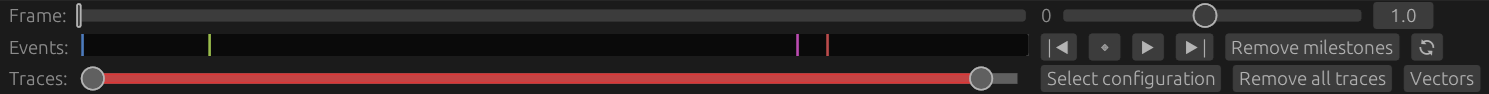
\includegraphics[width=\textwidth]{imagenes/panel_inf.png}
  \caption{Panel inferior de la representación temporal del \ac{C3D}}
  \label{fig:panel_inferior}
\end{figure}


Se distinguen tres filas. En la fila superior, en la parte izquierda aparece el \textit{frame} actual, representado mediante un \textit{slider}, que se puede mover para variar el \textit{frame}, y un número, ubicado justo a su derecha. Adicionalmente, a la derecha aparece otro \textit{slider} que permite ajustar la velocidad de reproducción de los eventos.

La segunda fila está dedicada a los eventos del \ac{C3D} (no confundir con los eventos de \textit{Bevy}), que son un parámetro dentro del fichero \ac{C3D} que permite fijar momentos importantes en el tiempo. Los eventos se pueden utilizar para navegar a través de estos momentos clave gracias a los botones de la parte derecha, que de izquierda a derecha significan: retroceder al evento anterior, marcar el \textit{frame} actual como un evento, variar entre pausa y reproducción, avanzar al evento siguiente, eliminar eventos y eliminar los eventos marcados por el usuario, dejando solo los eventos originales del \ac{C3D}.

Para diferenciar los eventos de \textit{Bevy} y los eventos del \ac{C3D}, se ha renombrado a estos últimos como \textit{milestones} (\textit{hitos}).

La última fila contiene un \textit{slider} que permite variar el rango de las trazas, \todo{Añadir cosas de trazas} variar entre configuraciones y ver u ocultar vectores, que se explican a continuación.

\section{Fichero de configuración \acs{TOML}}

El fichero de configuración de este proyecto define el modo de representación del fichero \ac{C3D} en el entorno 3D. 

Al igual que en el fichero de configuración de Vicon, explicado en \autoref{sec:ficheros-configuracion}, se definen las posibles configuraciones entre corchetes. Cualquier configuración cuenta con un grupo de puntos visibles (\textit{visible\_points}), un grupo de uniones (\textit{joins}) y un grupo de vectores (\textit{vectors}).

Estos grupos son opcionales, y pueden aparecer en cualquier orden. En caso de no aparecer, el programa no los representará.

\subsection{Configuración básica}

Una posible configuración podría ser la siguiente:

\begin{lstlisting}[style=mystyle, caption={Ejemplo simple de un fichero de configuración}, label={lst:ajuste-simple}]
[config1]
  visible_points = [
    "LFHD", "RFHD", "RBHD", "LBHD"
  ]
  joins = [
    ["LFHD", "RFHD", "RBHD", "LBHD", "LFHD"]
  ]
\end{lstlisting}

En el \autoref{lst:ajuste-simple} se muestra una configuración sencilla, \texttt{config1}, que representa los marcadores \ac{LFHD}, \ac{RFHD}, \ac{RBHD} y \ac{LBHD} como puntos visibles. Después, se define una unión entre los cuatro marcadores. Para representar un cuadrado, se duplica el primer marcador, \ac{LFHD}, al final de la lista. De este modo, se cierra la unión entre los cuatro marcadores. Además, se puede apreciar que en el grupo de uniones aparece un corchete extra. Esto se debe a que el grupo se considera una lista de listas. Las listas hijas representan diferentes uniones, es decir, grupos independientes de marcadores que se unen entre sí.

Estos cuatro marcadores representan los puntos de la cabeza. Es una combinación muy común, que posiblemente se utilice en varias configuraciones. Para facilitar su uso, el fichero de configuración permite definir un grupo de marcadores como un alias. De este modo, se puede definir el grupo de marcadores de la cabeza como \texttt{head}, y usarlo en la configuración de la siguiente manera:

\begin{lstlisting}[style=mystyle, caption={Ejemplo de un grupo de puntos}, label={lst:grupos-puntos}]
[point_groups]
  head = ["LFHD", "RFHD", "RBHD", "LBHD", "LFHD"]
  shoulders = ["LSHO", "RSHO"]

[config1]
  visible_points = [
    ["head"]
  ]
  joins = [
    [["head"]]
  ]
[config2]
  visible_points = [
    ["head"], ["shoulders"]
  ]
  joins = [
    [["head"]], 
    [["shoulders"]]
  ]
\end{lstlisting}

En el \autoref{lst:grupos-puntos} se muestra un ejemplo de cómo definir grupos de puntos, mediante la palabra reservada \textit{point\_groups}. En este caso, se definen dos grupos, \texttt{head} y \texttt{shoulders}. La forma de indicar al programa que se está referenciando a un grupo de puntos en vez de a un marcador es envolviendo al nombre entre corchetes.

En este caso, en la configuración \texttt{config1}, se representa el grupo de la cabeza como un punto visible y como una unión\footnote{Nótese que al usar el grupo de puntos de la cabeza, se está incluyendo dos veces el punto \ac{LFHD}. Esto no es relevante, dado que internamente el programa trata este punto como uno solo, al usarse como clave de un \textit{Hashmap}, que no permite la duplicación de elementos.}. En la configuración \texttt{config2}, se representan ambos grupos como puntos visibles y como uniones independientes. 

\subsection{Personalización general: Color y tamaño}

El fichero de configuración permite personalizar la representación de los marcadores. Para ello, se definen una serie de palabras reservadas. Estas palabras son \texttt{point\_color}, \texttt{point\_size}, \texttt{join\_color} y \texttt{line\_thickness}. Estas palabras son opcionales, y permiten personalizar la representación de los marcadores y las uniones. Los colores se pueden definir en formato rgb, como una lista de tres números enteros entre 0 y 255, o como rgb con transparencia, como una lista de cuatro números enteros entre 0 y 255.

\begin{lstlisting}[style=mystyle, caption={Configuración personalizada}, label={lst:cfg-personalizada}]
[point_groups]
  head = ["LFHD", "RFHD", "RBHD", "LBHD", "LFHD"]
  shoulders = ["LSHO", "RSHO"]

[config1]
  visible_points = [
    ["head"]
  ]
  joins = [
    [["head"]]
  ]
  point_color = [255, 0, 0]
  join_color = [0, 0, 255]
  line_thickness = 2.0
  point_size = 1.5

[config2]
  visible_points = [
    ["head"], ["shoulders"]
  ]
  joins = [
    [["head"]], 
    [["shoulders"]]
  ]
  point_color = [0, 0, 255, 100]
  point_size = 2.0
\end{lstlisting}

En el \autoref{lst:cfg-personalizada} se muestra un ejemplo de la personalización de una configuración, sobreescribiendo los valores por defecto. En este caso, para la configuración \texttt{config1}, los marcadores se representan en rojo, y las uniones en verde. Cada línea se representa con el doble de grosor que el valor por defecto, y los marcadores tienen un tamaño 1.5 veces mayor que el valor por defecto. En la configuración \texttt{config2}, los marcadores se representan en azul, con un 40\% de transparencia, y el doble de tamaño que el valor por defecto. Las uniones no se personalizan, por lo que se usan los valores por defecto.

Lo visto en el \autoref{lst:cfg-personalizada} es un ejemplo de sobreescritura de los valores por defecto para cada configuración. Sin embargo, se puede lograr una personalización más extrema gracias a los grupos de puntos, a los que se les pueden aplicar las mismas palabras reservadas. De este modo, se pueden definir diferentes colores y tamaños para cada grupo de puntos. En el \autoref{lst:cfg-grupos-personalizados} se muestra un ejemplo de cómo personalizar los grupos de puntos:

\begin{lstlisting}[style=mystyle, caption={Configuración personalizada de grupos de puntos}, label={lst:cfg-grupos-personalizados}]
[point_groups]
  head = ["LFHD", "RFHD", "RBHD", "LBHD", "LFHD"]
  shoulders = ["LSHO", "RSHO"]

[head.config]
  point_color = [255, 0, 0]
  point_size = 0.5
  join_color = [255, 128, 0]

[config1]
  visible_points = [
    ["head"]
  ]
  joins = [
    [["head"]]
  ]
  point_color = [255, 0, 0]
  join_color = [0, 0, 255]
  line_thickness = 2.0
  point_size = 1.5

[config2]
  visible_points = [
    ["head"], ["shoulders"]
  ]
  joins = [
    [["head"]], 
    [["shoulders"]]
  ]
  point_color = [0, 0, 255, 100]
  point_size = 2.0
\end{lstlisting}

Como se puede apreciar, se utiliza el nombre del grupo de puntos seguido de \texttt{.config} para definir la configuración de ese grupo, sobreescribiendo el valor por defecto de su configuración. En este caso, el grupo de puntos \texttt{head} se representa en rojo, con un tamaño de 0.5 veces el valor por defecto, y las uniones en naranja. El grupo de puntos \texttt{shoulders} no se personaliza, por lo que se usan los valores por defecto, que será azul en \texttt{config1} y verde en \texttt{config2}, puesto que verde es el color por defecto para las uniones, y en \texttt{config2} no se está sobreescribiendo.

\subsection{Personalización avanzada: Formas}

Las uniones entre dos marcadores se generan por defecto mediante un cilindro delgado, con apariencia de una línea. Mediante la palabra reservada \texttt{line\_thickness} se puede modificar este comportamiento, pero adicionalemente se puede modificar la forma. Las otras figuras admitidas son: un cono, un semicono y un prisma rectangular.

\begin{lstlisting}[style=mystyle, caption={Uso de formas}, label={lst:cfg-formas}] 
[config1]
  joins = [
    { points = ["RSJC", "RELJ"], shape = { type = "cone", radius = 1 } },
    { points = ["RELJ", "RWJC"], shape = { type = "semicone", radius1 = 4.0, radius2 = 2.0 } },
    { points = ["LSJC", "LELJ", "LWJC"], shape = { type = "prism", width = 4.0, height = 2.0 } },
  ]
\end{lstlisting}

Cada forma dispone de sus propias palabras reservadas, y las mayúsculas son irrelevantes (\textit{Case insensitive}). 

En el caso del cono, solo se debe especificar el radio, que define el tamaño de la circunferencia del primer elemento de la unión (en este caso \texttt{RSJC}). Además, cada forma tiene sinónimos, esto es, palabras que significan lo mismo para el programa. En el caso de ``cone'', se puede especificar también en español (``cono'').

En el caso del semicono, se deben especificar dos radios, que definen el tamaño de las dos circunferencias. Además, sinónimos de ``semicone'' son: ``semicono'', ``cone frustum'', ``cono truncado'', ``partial cone'', ``cono parcial'', ``truncated cone'' y ``cono truncado''.

\subsection{Configuración de vectores}

Los vectores son similares a los vectores de referencia explicados en \autoref{sec:bevy}. En el fichero de configuración, se definen como un punto de anclaje, una lista de elementos anclados a ese marcador, y opcionalmente una escala. Los vectores permiten representar relaciones espaciales y se pueden utilizar para definir trayectorias o movimientos en el espacio tridimensional.

\begin{lstlisting}[style=mystyle, caption={Configuración de un vector}, label={lst:cfg-vector}]
[config1]
  vectors = [ 
    ["OBJ1", "LVelOBJ1"],
    ["LUarmCM", ["LUarmIv", "LUarmJv", "LUarmKv"], 2.5],
    ["RUarmCM", ["RUarmIv", "RUarmJv"], 2.5],
    ["RUarmCM", "RUarmKv", 1.5],
]
\end{lstlisting}

En el \autoref{lst:cfg-vector} se muestra un ejemplo de como configurar vectores. En este caso, se han definido tres puntos de anclaje: \texttt{OBJ1}, \texttt{LUarmCM} y \texttt{RUarmCM}. 

El primero de ellos, \texttt{OBJ1}, tiene un solo elemento anclado, \texttt{LVelOBJ1}. Esta configuración ancla el marcador de representación de la velocidad de LVelOBJ1 a OBJ1. Esto representará un vector tangente a la trayectoria del objeto en cualquier punto.

El segundo, \texttt{LUarmCM}, tiene tres elementos anclados, \texttt{LUarmIv}, \texttt{LUarmJv} y \texttt{LUarmKv}, y una escala de 2.5. Esta es una configuración estándar para la representación de un sistema de coordenadas local, que sirven para cuantificar la rotación de un marcador.

El tercero, \texttt{RUarmCM}, tiene tres elementos anclados, \texttt{RUarmIv} y \texttt{RUarmJv}, con una escala de 2.5, y posteriormente se añade el tercer elemento, \texttt{RUarmKv}, con una escala de 1.5. Similar al caso anterior, se representa un sistema de coordenadas local, pero reduciendo el tamaño de la componente K.

Los vectores tienen una configuración de color fija. Para los vectores que tienen un número diferente a tres elementos anclados, se representan en amarillo, mientras que si el número de marcadores anclados a un punto es exactamente igual a tres, el programa entiende que se trata de una representación de vectores de referencia, para lo que utiliza colores estándar en otros motores de videojuegos, representando la primera componente en rojo, la segunda en verde y la tercera en azul. 

\subsection{Expresiones regulares}

A la hora de leer el fichero de configuración, se utilizan expresiones regulares para determinar si un marcador debe representarse o no. Esto permite representar un grupo de marcadores sin necesidad de definirlos uno a uno. Sin embargo, esto podría causar que se añadan más marcadores de los deseados. Por ejemplo, si se incluye el marcador \texttt{OBJ1}, se podría incluir también \texttt{LVelOBJ1}. 

Para evitar esto, el programa rodea el nombre del marcador con el símbolo \texttt{\^} al principio y el símbolo \texttt{\$} al final. De este modo, se asegura que el nombre del marcador coincide exactamente con el nombre del marcador en el fichero \ac{C3D}. Pero podría darse el caso de que se quiera representar ambos marcadores. Para ello, el programa admite un guión bajo (\texttt{\_}) como comodín. De este modo, si se incluye el marcador \texttt{\_OBJ1}, se incluirán todos los marcadores que cumplan la expresión regular, como \texttt{OBJ1} o \texttt{LVelOBJ1}. 

\section{Carga de ficheros}

El fichero de configuración y el fichero \ac{C3D} se cargan de forma simple, arrastrando el fichero a la ventana del programa. El programa detecta el tipo de fichero y lo carga automáticamente. Se puede variar el fichero \ac{C3D} o el fichero de configuración en tiempo de ejecución, y el programa lo detecta automáticamente.

\textit{Bevy} tiene una función nativa para la captura de los ficheros que se sueltan sobre la ventana. Sin embargo, en la versión web el navegador captura el fichero antes que \textit{Bevy}, por lo que es imposible la carga de ficheros de este modo. Para ello se ha modificado el crate \texttt{bevy\_web\_file\_drop} para darle compatibilidad con la versión 0.15 de \textit{Bevy}, dado que este \textit{crate} está escrito para la versión 0.14 y no presenta compatibilidad \autocite{Bevy_web_file_dropCratesioRust2024}.

Con estas modificaciones, el programa es capaz de capturar un archivo tanto en la versión de escritorio como en la versión web. Para esta última utiliza una \textit{Blob URL} para la carga del fichero \autocite{AnswerWhatBlob2015,FileAPI}.

Cuando un fichero se carga, se toman diferentes acciones, dependiendo de su tipo. Si se trata de un \ac{C3D} se eliminan todos los marcadores y se envía un evento de carga al \textit{parser} de \ac{C3D}. Este \textit{parser} se encarga de cargar el fichero y enviar un evento al programa con los datos cargados. Si se trata de un fichero de configuración, simplemente se indica al programa que debe generar nuevamente las uniones y vectores, sin necesidad de eliminar los marcadores. 

\section{Representación tridimensional} 

\subsection{Representación de los marcadores} \label{sec:representacion-marcadores}

Los marcadores se representan como esferas, y se pueden personalizar mediante el fichero de configuración. Internamente, el programa utiliza dos estructuras de datos, una contiene el nombre del marcador y su visibilidad, y la otra es una agrupación de marcadores, siguiendo el patrón \ac{ECS} de \textit{Bevy}. Es decir, el componente \texttt{Marker} contiene el nombre del marcador y su visibilidad, mientras que el componente \texttt{C3dMarkers} es únicamente una asignación de una estructura vacía a todos los marcadores. Esto permite eliminar todos los marcadores de forma sencilla, eliminando únicamente el componente padre.

Es necesario mantener en memoria todos los marcadores, incluso los que no son visibles según el fichero de configuración. Esto se debe a que el programa permite cambiar la configuración en tiempo de ejecución, y por tanto, es necesario mantener todos los marcadores en memoria para poder representarlos. Sin embargo, el programa no los representa si no son visibles, gracias a que la estructura de datos contiene la visibilidad de cada marcador\footnote{\textit{Bevy} entiende la visibilidad de cualquier entidad como un enumerado, que puede ser visible, invisible o heredado.}.

Si se ejecuta el programa sin un fichero de configuración, se representan todos los marcadores como visibles. Esto permite comprobar que el \textit{parser} de \ac{C3D} funciona correctamente, y que se están cargando todos los marcadores. Sin embargo, no se recomienda su uso, dado que el número de marcadores puede ser elevado, y la representación muestra datos que no tienen un sentido espacial. En la \autoref{fig:marcadores} se muestra una imagen de la representación de los marcadores sin un fichero de configuración. Se puede observar que el número de marcadores es elevado, y que aparecen marcadores que no tienen un sentido espacial, como un vector de velocidad. La \autoref{fig:marcadores} resalta la importancia de la configuración, puesto que es inviable el estudio de un movimiento con un número tan elevado de marcadores. 

\begin{figure}[H]
  \centering
  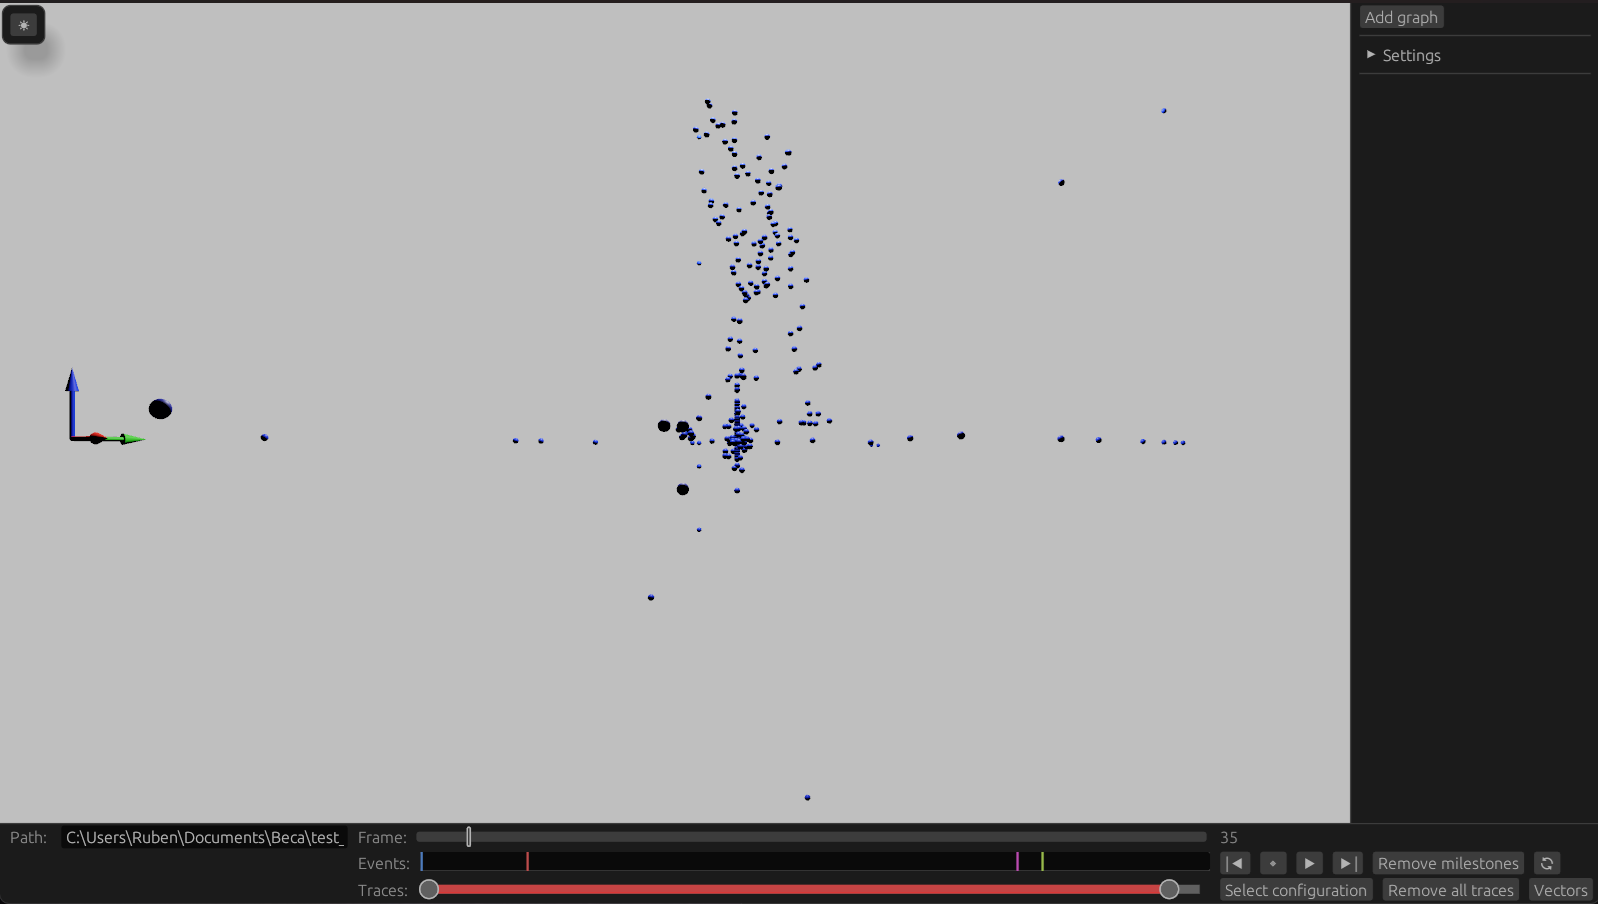
\includegraphics[width=\textwidth]{imagenes/marcadores.png}
  \caption{Representación de marcadores del \ac{C3D} sin un fichero de configuración}
  \label{fig:marcadores}
\end{figure}

Para representar los marcadores, el programa utiliza un componente de \textit{Bevy} llamado \texttt{Mesh}. Este componente permite representar una malla en el espacio tridimensional. En este caso, se utiliza una esfera como malla, con un tamaño y color definidos en el fichero de configuración, o en su defecto, en color azul y con un tamaño por defecto. Si se ha cargado un fichero de configuración, cada marcador se considera visible si aparece en el grupo de puntos visibles. En caso contrario, se considera invisible. De este modo, es sencillo representar solo una parte de los marcadores, y ocultar el resto.

\begin{figure}[H]
  \centering
  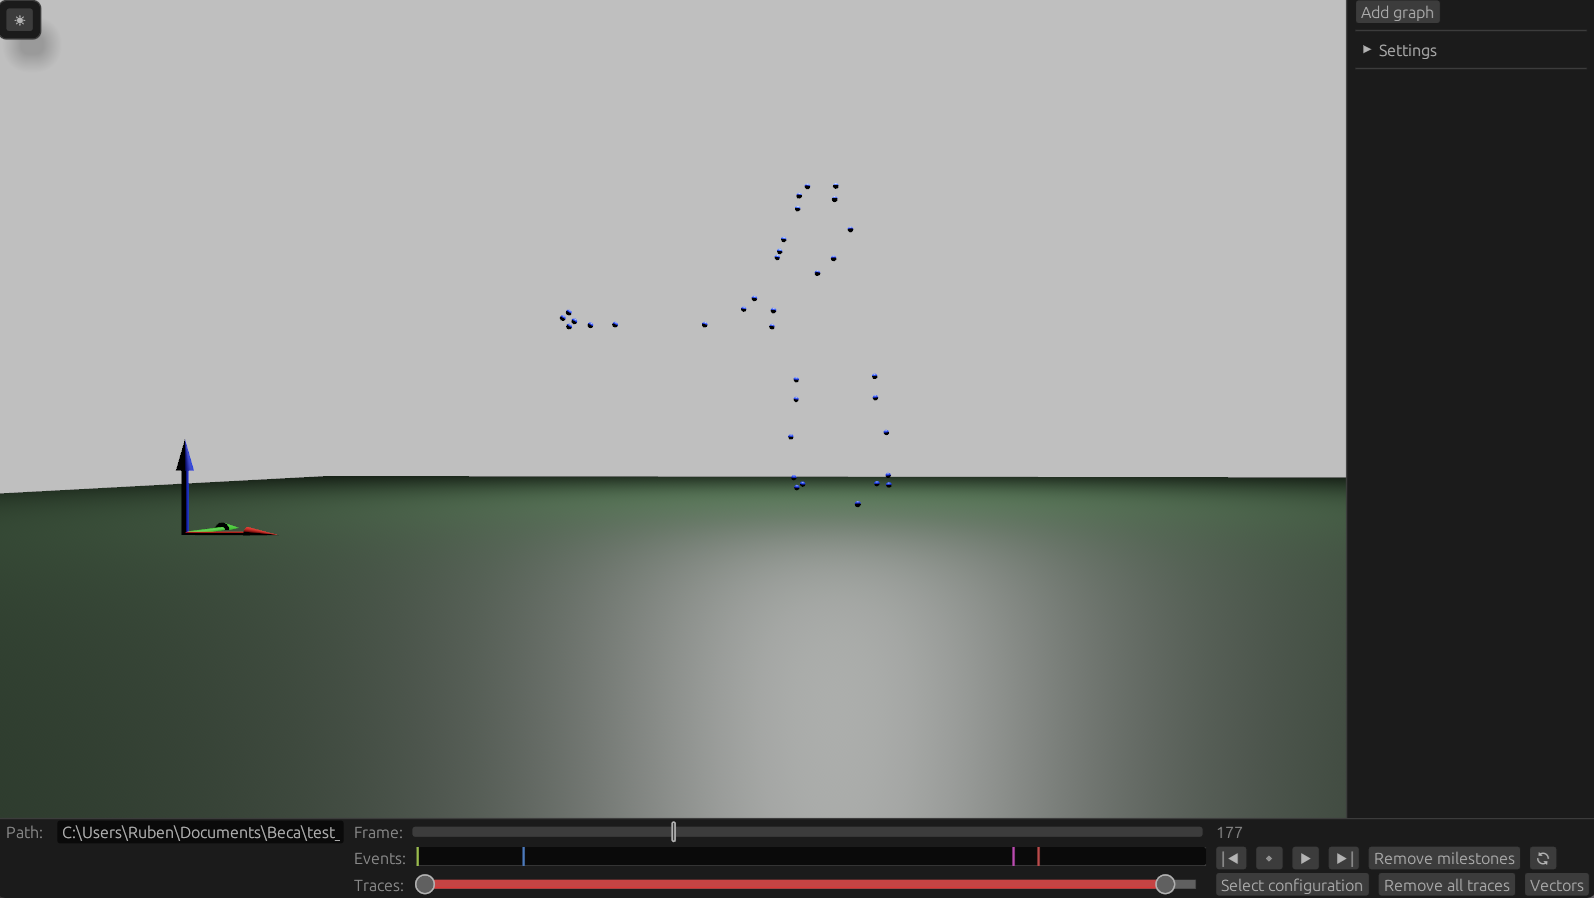
\includegraphics[width=\textwidth]{imagenes/config-basica.png}
  \caption{Representación de marcadores del \ac{C3D} con un fichero de configuración}
  \label{fig:cfg-basica}
\end{figure}

La \autoref{fig:cfg-basica} muestra el mismo fichero que la \autoref{fig:marcadores}, pero filtrando la mayoría de puntos para generar un avatar.

\subsection{Representación de las uniones} \label{sec:representacion-uniones}

Las uniones se representan como figuras entre marcadores. Estas figuras pueden ser de diferentes tipos, como un cilindro, un cono, un semicono o un prisma rectangular. 




\subsection{Velocidad de reproducción}

El programa admite dos modos de funcionamiento, velocidad fija o velocidad adaptativa. 

El primer modo es ideal para el estudio de un movimiento con la mayor precisión, esto es, representando la velocidad real de la captura del movimiento, utilizando la tasa de refresco del \ac{C3D}. En caso de que la tasa de refresco de la pantalla sea inferior a la tasa de refresco del \ac{C3D}, \textit{Bevy} realiza una interpolación para que la velocidad de reproducción sea la del \ac{C3D}. Por ejemplo, para una tasa de refresco de una pantalla de 60 Hz representando un movimiento de 240 Hz, \textit{Bevy} representará uno de cada cuatro fotogramas del \ac{C3D}. Además, este modo permite variar la velocidad de reproducción, entre 0.1 y 2.0 veces la tasa de refresco del \ac{C3D}. 

Por el contrario, el segundo modo es ideal para el estudio del movimiento con la mayor calidad, es decir, sin perder información sobre los fotogramas. En este modo, no se tiene en cuenta la tasa de refresco del \ac{C3D}, \textit{Bevy} representará el fichero respetando las limitaciones del \textit{hardware}. Esto es, si se dispone de una pantalla de 60 Hz, como máximo el programa se actualizará a esta velocidad (aunque si hay un componente más restrictivo, por ejemplo una tarjeta gráfica incapaz de dar una tasa de refresco adecuada, se respetará esta limitación).

% \section{Configuración de la cámara} \label{sec:cfg-camara}
